\chapter{\MakeUppercase{Working Principle}}
\setcounter{equation}{0}

\section{\MakeUppercase{Motivation and Objectives}}
The core motivation for the proposed method stems from the observation that training Neural Radiance Fields (NeRFs) with an abundance of blurry and imbalanced data leads to a measurable decrease in performance. Specifically, the ablation study indicates that utilizing the entire blurred image dataset slightly reduces performance. To address the dual challenges of optimal data selection and data imbalances—particularly those arising from light-field camera geometry and varying degrees of blur—the authors employ a pool-based active learning framework. The primary objective is to intelligently select the most informative, least-blurred samples from the input pool for labeling and training, thereby enhancing the accuracy and robustness of the NeRF model compared to conventional training on the full, imperfect dataset.

\section{\MakeUppercase{Classification of Labeled and Unlabeled Datasets}}
To ensure an efficient and effective training process, the authors utilize active learning to classify and prepare the input images into an initial labeled dataset ($D_L$) and an unlabeled dataset ($D_U$).\cite{bib14}

\subsection{\MakeUppercase{Light Field Camera Position}}
To construct an effective labeled set, it is crucial to select initial images that are helpful and to account for the inherent imbalance among camera positions in light-field type data. Images captured from camera positions distant from the light field center are prone to occlusions at their outer edges during restoration. To mitigate this, the authors calculate the distances ($d_i$) of each camera position's coordinates ($x_i, y_i, z_i$), obtained from COLMAP, relative to the average camera position coordinates (x, y, z) across all $N$ images using the equation:
\[
    d_i = \sqrt{\left(x_i - x\right)^2 \text{+} \left(y_i - y\right)^2 \text{+} \left(z_i - z\right)^2}, \quad i = 1, \ldots, N.
\]
The images are then initially included in the labeled dataset ($D_L$) based on a balanced distribution of these distances, thereby minimizing initial camera-induced artifacts.

\subsection{\MakeUppercase{Entropy for Blur Images}}
The authors further refine the selection for $D_L$ by using entropy to quantify the amount of information within each image and select only the data that is most likely to improve model performance. High-quality, sharp images exhibit larger entropy values, while low-quality, blurred images possess smaller entropy values. The blur entropy for each image is calculated as the sum of local entropies:
\begin{figure}[htbp]
    \centering
    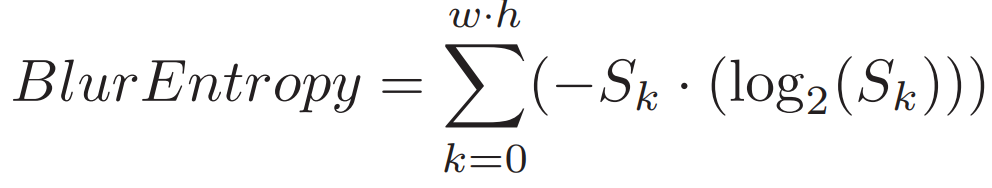
\includegraphics[width=0.47\linewidth]{assets/figures/eq2.png}
\end{figure}
\noindent where $S_k$ is the local entropy at window $k$, and $w$ and $h$ are the width and height of the image. The images selected based on the light field camera candidates are combined with these blur entropy values and updated into $D_L$, typically prioritizing less-blurred (higher entropy) images.

\subsection{\MakeUppercase{Unseen View Camera Poses}}
To address the lack of ambient view information at the outer edges of the forward-facing light field images, and to overcome the limitations of a static dataset, the authors generate unseen view camera poses. This is achieved by manipulating the rotation and translation values of the camera extrinsics derived from COLMAP outputs. These generated unseen view camera poses, along with the camera poses of the strongly blurred original images, are assigned to the unlabeled set ($D_U$).

\section{\MakeUppercase{Deblur-NeRF Network}}

The base of the authors' method is the Deblur-NeRF Network, which extends the standard Neural Radiance Field (NeRF) formulation to integrate simultaneous deblurring with novel view synthesis. Standard NeRF maps 3D coordinates $\mathbf{x}=(x, y, z)$ and 2D viewing directions $\mathbf{d}=(\theta, \phi)$ to color $\mathbf{c}$ and density $\sigma$ using a Multi-Layer Perceptron (MLP) $F_{\Theta}$. NeRF significantly improves performance by calculating volume-rendering integrals to represent the output colors of the pixels. To handle blurred inputs, Deblur-NeRF extends 2D spatial deblurring to 3D ray deblurring through a Deformable Sparse Kernel (DSK) module. This module generates canonical kernel rays at sparse kernel points within a window $N(\mathbf{p})$ around the primary ray $\mathbf{p}$ for a given pixel location $(x, y)$. The NeRF model is then trained with an optimized, deblurred ray by combining the ray weight and the corresponding sharp colors from the canonical kernel rays. This entire process is initially trained using data from the labeled pool ($D_L$).

\section{\MakeUppercase{Optimization Using Active Learning}}
To combat the performance degradation caused by abundant blurry and imbalanced data, the authors employ a pool-based active learning strategy for optimization. After the initial training of the NeRF and DSK modules using the labeled pool ($D_L$), the authors utilize the trained model to perform image reconstruction through deblurring on the data in the unlabeled pool ($D_U$).

The key step for querying new data is employing the uncertainty sampling method based on entropy calculations. The authors calculate the entropy of the reconstructed (deblurred) images from the $D_U$ pool to select the sharpest, most suitable samples (those with the highest entropy) for querying and labeling. These selected samples are then integrated into the labeled pool ($D_L$).\cite{bib13}

The NeRF model is subsequently trained from scratch with the newly integrated labeled data. Importantly, since the newly integrated data have been effectively deblurred and selected for high information content, the performance is further improved even when training only the NeRF model (excluding the DSK module) during the subsequent optimization cycles. This iterative process continues until a satisfactory level of model performance is achieved (estimated to be about half of the total training time).
\section{\MakeUppercase{Framework}}
\begin{figure}[htbp]
    \centering
    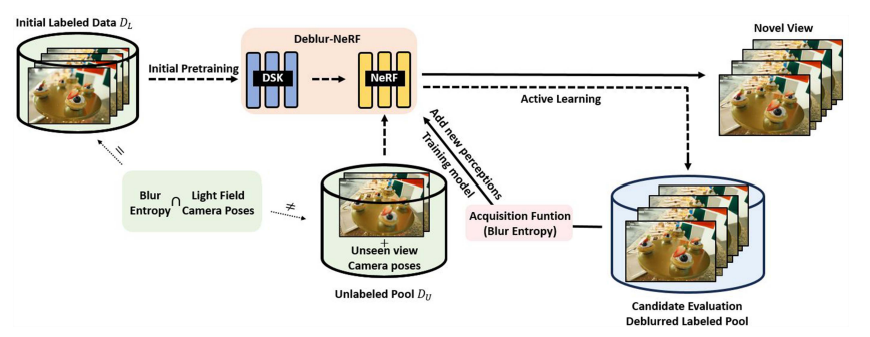
\includegraphics[width=1.00\linewidth]{assets/Images/framework.png}
    \caption{NeRF-DA framework reproduced from the supplied report of Hong and Kim.\cite{bib1}}
\end{figure}
The initial labeled set $D_L$ has high entropy on the blurred images and comprises images that ensure that the camera position is not on the outer edge to maintain data balance. Then, the authors utilize $D_L$ to train the Deblur-NeRF model, which comprises the DSK module for deblurring and the NeRF module for view synthesis, to establish a strong foundation for deblurring. We construct an unlabeled set $D_U$ comprising strongly blurred images not present in the initial $D_L$ and additional unseen view camera poses, introduced to maintain balance, then reconstruct sharp images using the model. As in pool-based active learning, we conduct NeRF training by employing entropy to select the optimal sample for querying within the unlabeled pool $D_U$.

\section{Step-by-Step Summary}
\begin{enumerate}
\item Obtain camera poses and assess the information content of the input images.
\item Build an initial selected pool and a candidate pool, including additional camera poses.
\item Train the Deblur-NeRF model on the selected images.
\item Reconstruct candidate views and evaluate their information content.
\item Add selected reconstructed views and train the NeRF on the expanded pool.
\item Render sharp novel views and evaluate reconstruction quality.
\end{enumerate}
The process above describes the selected paper's approach.\cite{bib1}
